

\setchapterpreamble[c][.7\textwidth]{\itshape\dgrau\small
    In diesem Vortrag werden grundlegende Eigenschaften und Operationen von Mengen vorgestellt. Ebenso werden Familien und Tupel eingeführt, da sie grundlegend für die Konzepte „Relation“, „Folge“ und „Verknüpfung“ aus den späteren Vorträgen sind.
\vspace{24pt}}

    
\chapter{Mengen und Familien}


\section{Mengen und Elemente}


Der Begriff der Menge wurde bereits im Vortrag über Logik in \cref{mengenimlogikkapitel} angesprochen. Seine Einführung in die Mathematik erfolgte durch Georg Cantor\footnote{\href{https://de.wikipedia.org/wiki/Georg_Cantor}{Georg Cantor (1845-1918)}} in den 1870er Jahren. Cantor beschreibt seine Idee in \cite{Can95} mit den folgenden Worten:


\begin{de}[Mengendefinition von Cantor] \label{def:menge} \index{Menge}
    „Unter einer \textbf{Menge} $M$ verstehen wir jede Zusammenfassung von bestimmten wohlunterschiedenen Objekten $m$ unserer Anschauung oder unseres Denkens (welche die \textbf{Elemente} von $M$ genannt werden) zu einem Ganzen.“
\end{de}


\begin{bem}
    Eine (möglicherweise fiktive) Anekdote aus \cite{Ded32}, S. 449 beschreibt folgende „Veranschaulichungen“ des Mengenbegriffs:
    \begin{quote}
        Dedekind\footnote{\href{https://de.wikipedia.org/wiki/Richard_Dedekind}{Richard Dedekind (1831-1916)}} äußerte, hinsichtlich des Begriffes der Menge: er stelle sich eine Menge vor wie einen geschlossenen Sack, der ganz bestimmte Dinge enthalte, die man aber nicht sähe, und von denen man nichts wisse, außer dass sie vorhanden und bestimmt seien. Einige Zeit später gab Cantor seine Vorstellung einer Menge zu erkennen: Er richtete seine kolossale Figur hoch auf, beschrieb mit erhobenem Arm eine großartige Geste und sagte mit einem ins Unbestimmte gerichteten Blick: „Eine Menge stelle ich mir vor wie einen Abgrund.“
    \end{quote}
\end{bem}


\begin{nota}[Elementzeichen]
    Seien $M$ eine Menge und $x$ irgendein Objekt. Man schreibt
    \begin{align*}
        x  \in M \qquad&:\Leftrightarrow\qquad \text{$x$ ist ein Element von $M$} && (\text{lies: „$x$ in $M$“})\\
        x\notin M \qquad &:\Leftrightarrow\qquad \text{$x$ ist kein Element von $M$} && (\text{lies: „$x$ nicht in $M$“})
    \end{align*}
    Das Symbol „$\in$“ bezeichnet ein zweistelliges Prädikat im Sinne von \cref{def:praedikat}.
\end{nota}


\begin{axiom}[Extensionalitätsaxiom] \label{mengengleich} \index{Extensionalitätsaxiom}
    Zwei Mengen $M,N$ stimmen genau dann überein, wenn sie dieselben Elemente haben. Als Formel:
        \[ (\forall x:\quad x\in M\ \leftrightarrow\ x\in N)\qquad\leftrightarrow\qquad M=N\]
    Dementsprechend sind zwei Mengen \emph{verschieden}, wenn mindestens eine der beiden ein Element enthält, das die andere nicht enthält.
\end{axiom}


\begin{de}[Extension einer Eigenschaft] \label{def:extension} \index{Extension (einer Eigenschaft)}
    Sei $E(x)$ eine Eigenschaft. Die Menge aller Objekte mit der Eigenschaft $E$ ist wegen des Extensionalitätsaxioms \cref{mengengleich} eindeutig bestimmt. Sie heißt die \textbf{Extension}\footnote{vgl. \cref{extensionimlogikkapitel}} von $E$ und wird notiert durch
    \begin{align*}
        \{ x\mid E(x) \} && (\textnormal{lies: „Menge aller $x$, für die gilt: $E(x)$“})
    \end{align*}
    Per Definition gilt:
        \[ \forall a:\qquad a\in \{x\mid E(x)\} \ \leftrightarrow\ E(a) \]
    Für eine Menge $M$ von Objekten vom Typ der Variablen $x$ wird durch
        \[ \{ x\in M\mid E(x) \} := \{ x\mid x\in M\ \text{und}\ E(x)\} \]
    die Menge aller Elemente von $M$, die die Eigenschaft $E$ besitzen, notiert.
\end{de}


\begin{bsp} \label{bsp:extension}
    Das Konzept „Extension einer Eigenschaft“ erlaubt es, Mengen mittels Eigenschaften zu definieren. Zum Beispiel:
    \begin{enumerate}
        \item Es ist $\bbP := \{p\mid p\ \text{ist eine Primzahl}\}$ die Menge aller Primzahlen. Beispielsweise sind $23\in \bbP$ und $97\in\bbP$, denn $23$ und $97$ sind Primzahlen. Dagegen ist $91\notin \bbP$, denn $91$ ist keine Primzahl wegen $91=7\cdot 13$.
        \item Es ist $\{ x\mid x\ \text{liest dieses Vorkurs-Skript} \}$ die Menge aller Leser dieses Skripts. Zum Beispiel bist DU ein Element dieser Menge.
        \item Es ist $[0,1] := \{ x\in \R \mid 0\le x\le 1\}$ die Menge aller reellen Zahlen zwischen Null und Eins, das sogenannte (abgeschlossene) \emph{Einheitsintervall}.
        \item Es ist $Q:=\{ n\in \N \mid \exists m\in \N:\ n=m^2 \}$ die Menge aller Quadratzahlen. Beispielsweise sind $100\in Q$ und $529\in Q$, aber $12\notin Q$ und $1000\notin Q$.
    \end{enumerate}
\end{bsp}


\begin{nota}[Definition einer Menge durch Auflistung] \label{auflistung}
    Seien $n\in \N$ und $a_1,\dots , a_n$ eine Handvoll Objekte. Dann bezeichnet
        \[ \{a_1,\dots , a_n\} := \{ x\mid x=a_1\ \text{oder}\ x=a_2\ \text{oder}\ \ldots\ \text{oder}\ x=a_n \} \]
    diejenige Menge, die genau aus $a_1,\dots , a_n$ besteht. Auf diese Weise kannst du Mengen mit „wenigen“ Elementen schlicht durch Auflistung aller ihrer Elemente definieren.
\end{nota}


\begin{bsp}
    Zum Beispiel ist
        \[ M:=\{2,3,5,7,11,13,17,19,23,29,31,37,41,43,47,53,59,61,67,71,73,79,83,89,97\} \]
    diejenige Menge, die genau aus den Zahlen $2,3,5,\dots , 97$ besteht. Es gilt
        \[ M = \{p\mid p\ \text{ist eine Primzahl und}\ 1< p <100 \} \]
    d.h. $M$ ist die Menge aller Primzahlen zwischen $1$ und $100$. Sie enthält genau fünfundzwanzig Elemente.
\end{bsp}


\begin{bem}
    Gelegentlich werden auch Mengen mit unendlich vielen Elementen über eine Art „Auflistung“ definiert, zum Beispiel
        \[ M := \{1, 3, 5, 7, 9,\ldots \} \]
    Diese Art von „Definition“ setzt beim Leser das Erkennen eines intendierten Musters voraus und kann zu Missverständnissen führen. Im Zweifelsfall solltest du eine Definition durch eine Eigenschaft bevorzugen, in diesem Fall etwa
        \[ M := \{n \in \N \mid n\ \text{ist ungerade} \} \]
\end{bem}


\begin{nota}[*] \label{beschraenktquant}
    Seien $M$ eine Menge und $E$ eine Eigenschaft. Für Aussagen über die Elemente von $M$ gibt es folgende Schreibweisen\footnote{vgl. \cref{def:allquant}, \cref{def:existquant} und \cref{def:eindquant}}
    \begin{align*}
        \forall x\in M:\ E(x) \qquad :& \Leftrightarrow\qquad \forall x:\ (x\in M\ \to\ E(x))  \\
        (\text{lies: „Für jedes $x$ aus $M$ gilt $E(x)$“}) & \\[0.5em]
        \exists x\in M:\ E(x) \qquad :& \Leftrightarrow\qquad \exists x:\ (x\in M\ \land\ E(x))  \\
        (\text{lies: „Es gibt ein $x$ in $M$, für das $E(x)$ gilt“}) & \\[0.5em]
        \nexists x\in M:\ E(x) \qquad :& \Leftrightarrow\qquad \nexists x:\ (x\in M\ \land\ E(x))  \\
        (\text{lies: „Es gibt kein $x$ in $M$, für das $E(x)$ gilt“}) & \\[0.5em]
        \exists ! x\in M :\ E(x) \qquad :& \Leftrightarrow\qquad \exists ! x:\ (x\in M\ \land\ E(x)) \\ (\text{lies: „Es gibt genau ein $x$ in $M$, für das $E(x)$ gilt“})
    \end{align*}
    um auszudrücken, dass jedes/mindestens eines/keines/genau eines der Elemente von $M$ die Eigenschaft $E$ besitzt.
\end{nota}


\begin{bsp}[*]
    Es gilt:
    \begin{align*}
        \forall n\in \N &:\ n\cdot (n+1)\ \text{ist eine gerade Zahl} && (\text{vgl. \cref{bsp:fallunterscheidung}})\\
        \exists x\in \R &:\ x=x^5-1 && (\text{vgl. \cref{bsp:exverwendung}})\\
        \nexists n\in \N &:\ 17\cdot n = 198 && (\text{vgl. \cref{bsp:reductio}})\\ 
        \exists ! x\in \R \ \forall y\in \R & :\ xy=x &&(\text{vgl. \cref{bsp:eindbeweis}})
    \end{align*}
\end{bsp}





\section{Teilmengen}


\begin{de}[Teilmenge] \label{def:teilmenge} \index{Teilmenge}
    Seien $M$ und $N$ zwei Mengen.
    \begin{itemize}
        \item $M$ heißt eine \textbf{Teilmenge} (manchmal auch: \textbf{Untermenge}) von $N$ (und $N$ eine \textbf{Obermenge} von $M$), falls jedes Element von $M$ auch ein Element von $N$ ist. Notation:
        \begin{align*}
            M \subseteq N \qquad &:\Leftrightarrow\qquad M\ \text{ist eine Teilmenge von $N$} \\
            M \nsubseteq N \qquad &:\Leftrightarrow\qquad M\ \text{ist keine Teilmenge von $N$}
        \end{align*}
        \item $M$ heißt eine \textbf{echte Teilmenge} von $N$, falls $M$ eine Teilmenge von $N$ ist, aber von $N$ verschieden ist. Notation:
        \begin{align*}
            M\subsetneq N \qquad:\Leftrightarrow\qquad M\subseteq N\ \text{und}\ M\neq N
        \end{align*}
        Mit anderen Worten: Jedes Element von $M$ ist auch eines von $N$, wohingegen es mindestens ein Element von $N$ gibt, das keines von $M$ ist.
        \begin{figure}[ht]
            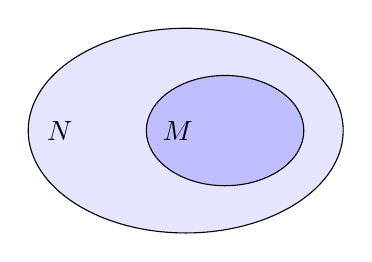
\begin{tikzpicture}
                \filldraw[fill=blue!10!white, draw=black] (0,0) ellipse (2cm and 1.3cm);
                \filldraw[fill=blue!25!white, draw=black] (.5,0) ellipse (1cm and .7cm);
                \path (-1.6,0) node {$N$} (-.1,0) node {$M$};
            \end{tikzpicture}
            \centering \caption{Die Menge $M$ ist Teilmenge der Menge $N$.}
        \end{figure}
    \end{itemize}
\end{de}


\begin{bsp} \quad
    \begin{enumerate}
        \item Es ist $\{m\mid m\ \text{ist ein Mensch}\}\subseteq \{t\mid t\ \text{ist ein Säugetier}\}$, da alle Menschen Säugetiere sind.
        \item Es ist $\Q\subsetneq \R$, da zwar jede rationale Zahl eine reelle Zahl ist, es aber auch irrationale reelle Zahlen, zum Beispiel $\sqrt{2}$, gibt.
    \end{enumerate}
\end{bsp}


\begin{nota}[Alternative Schreibweisen]
    Bisweilen werden in der Literatur auch abweichende Notationen benutzt: etwa $M\subseteq N$ für beliebige und $M\subset N$ für echte Teilmengen; oder aber $N\subseteq M$ für beliebige und $M\subsetneqq N$ für echte Teilemengen. Hier ist eine Liste verschiedener Konventionen:
    \[\begin{tabular}{c|ccc}
        & Teilmenge & echte Teilmenge \\ \hline
        Dieser Text & $\subseteq$ & $\subsetneq$ \\
        Alternative 1 & $\subseteq$ & $\subset$ \\
        Alternative 2 & $\subset$ & $\subsetneq$ oder $\subsetneqq$
    \end{tabular}\]
\end{nota}


\begin{bem}[Teilmengeninklusionen beweisen/widerlegen] \label{teilmengebeweisen}
    Seien $M,N$ zwei Mengen. Da es sich bei der Aussage „$M\subseteq N$“ um eine Allaussage handelt (\emph{jedes} Element von $M$ ist ein Element von $N$), kannst du sie mit der Technik aus \cref{allbeweis} beweisen: fixiere ein beliebiges Element von $M$ und zeige irgendwie, dass dies auch ein Element von $N$ ist.
    
    Wenn du meinst, dass „$M\subseteq N$” eine falsche Aussage ist, kannst du sie mit der Technik aus \cref{gegenbeispiel} widerlegen: finde ein Element von $M$, das kein Element von $N$ ist.
\end{bem}


\begin{satz}[* Eigenschaften von $\subseteq$]\label{teilmengeneig}
    Seien $L, M, N$ drei Mengen. Dann gilt:
    \begin{enumerate}
        \item $M\subseteq M$ (Reflexivität).
        \item Aus $L\subseteq M$ und $M\subseteq N$ folgt $L\subseteq N$ (Transitivität).
        \item Aus $M \subseteq N$ und $N\subseteq M$ folgt $M=N$ (Antisymmetrie).
    \end{enumerate}
    \begin{figure}[ht]
        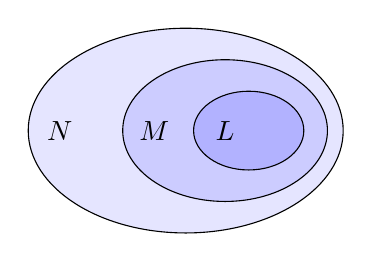
\begin{tikzpicture}
            \filldraw[fill=blue!10!white, draw=black] (0,0) ellipse (2cm and 1.3cm);
            \filldraw[fill=blue!20!white, draw=black] (.5,0) ellipse (1.3cm and .9cm);
            \filldraw[fill=blue!30!white, draw=black] (.8,0) ellipse (.7cm and .5cm);
            \path (-1.6,0) node {$N$} (-.4,0) node {$M$} (.5,0) node {$L$};
        \end{tikzpicture}
        \centering \caption{Illustration der Transitivität von „$\subseteq$“}
    \end{figure}
\end{satz}


\begin{bew}
    \begin{enumerate}
        \item Für alle Elemente $m\in M$ gilt per se schon $m\in M$, also ist $M$ in $M$ enthalten.\footnote{vgl. \cref{implikationref}: Jede Aussage impliziert sich selbst.}
        \item Sei $x\in L$ beliebig. Wegen $L\subseteq M$ gilt dann $x\in M$. Aus $x\in M$ folgt wegen $M\subseteq N$, dass auch $x\in N$. Da das Element $x\in L$ beliebig gewählt war, ist damit $L\subseteq N$ bewiesen.\footnote{Das war ein direkter Beweis mit Zwischenschritten, vgl. \cref{implikationtrans}:
            \[ x\in L\xrightarrow{L\subseteq N} x\in N \xrightarrow{N\subseteq M} x\in M \]}
        \item Wegen $M\subseteq N$ und $N\subseteq M$ ist jedes Element von $M$ auch eines von $N$ und umgekehrt. Mit anderen Worten: $M$ und $N$ haben genau dieselben Elemente. Aus dem Extensionalitätsaxiom \cref{mengengleich} folgt nun, dass $M=N$. \qed
    \end{enumerate}
\end{bew}


\begin{bem}[* Gleichheit von Mengen beweisen] \label{mengengleichbeweis}
    Kombinieren von \cref{teilmengebeweisen} und \cref{teilmengeneig}(c) liefert eine Methode, die Gleichheit zweier Mengen $M,N$ zu zeigen, indem nacheinander die Inklusion $M\subseteq N$ und die Inklusion $N\subseteq M$ gezeigt werden.
    
    Aus beiden Inklusionen folgt dann mit \cref{teilmengeneig}(c), dass $M=N$. In Beweisen solltest du die Abschnitte, die den einzelnen Inklusionen $M\subseteq N$ und $N\subseteq M$ gewidmet sind, durch Markierungen deutlich machen.
    
    Diese Beweistechnik ist auch Inhalt von \cref{aufg:capcupgesetze} .
\end{bem}


\begin{bsp}[*] \label{bsp:mengengleichbeweis}
    Es ist $\{1,2,3\}=\{1,1,3,2\}$.
\end{bsp}


\begin{bew}
    \begin{itemize}
        \item[„$\subseteq$“] Sei $x\in\{1,2,3\}$, also $x=1$, $x=2$ oder $x=3$. In jedem dieser Fälle\footnote{vgl. \cref{auflistung} und \cref{fallunterscheidung}} gilt auch $x\in\{1,1,3,2\}$.
        \item[„$\supseteq$“] Sei umgekehrt $x\in\{1,1,3,2\}$,  also $x=1$, $x=1$, $x=3$ oder $x=2$. In jedem dieser Fälle gilt auch $x\in\{1,2,3\}$. \qed
    \end{itemize}
\end{bew}


\begin{bem} \label{mengenstrukturlos}
    Im letzten Beispiel sehen wir ganz deutlich, dass die Elemente einer Menge keiner Reihenfolge oder „Zählung“ unterliegen: Eine Menge trägt von sich aus bis auf ihre Elemente keine weitere Struktur; Fragen wie „Wie genau / Wie oft / An welcher Stelle ist $x$ in $M$ enthalten?“ kann sie also nicht beantworten, sondern nur „Ist $x$ in $M$ enthalten (oder nicht)?“.
    
    Möchte man den Elementen dennoch verschiedene „Plätze“ zuweisen, bietet sich der Begriff der „Familie“ an, der später in \cref{def:familie} eingeführt wird.
\end{bem}





\section{Die leere Menge}


\begin{de} \index{Leere Menge} \index{Einermenge}
    Eine Menge heißt
    \begin{itemize}
        \item \textbf{leer}, wenn sie gar keine Elemente enthält.
        \item \textbf{nichtleer}, wenn sie nicht leer ist.\footnote{Im Englischen nennt man eine Menge auch ``\href{https://en.wikipedia.org/wiki/Inhabited_set}{inhabited}'', wenn sie mindestens ein Element enthält.}
        \item eine \textbf{Einermenge} (englisch: ``singleton''), wenn sie genau ein Element enthält, also von der Form $\{x\}$ für irgendein Objekt $x$ ist.
    \end{itemize}
\end{de}


\begin{satz} \label{leeremengeeind}
    Es gibt genau eine leere Menge.
\end{satz}


\begin{bew}
    (Existenz): Sei $E(x)$ irgendeine Eigenschaft, die kein einziges Objekt besitzt (z.B. „$x\neq x$“). Dann ist $\{ x\mid E(x) \}$ eine leere Menge. \\[0.5em]
    (Eindeutigkeit): Seien $M,N$ zwei leere Mengen. Dann enthalten $M$ und $N$ genau dieselben Elemente (nämlich gar keine), sodass aus \cref{mengengleich} folgt, dass $M=N$.
\end{bew}


\begin{nota}[\textbf{Die} leere Menge]
    Somit ergibt es Sinn, von \emph{der} leeren Menge zu sprechen. Die leere Menge wird meist notiert durch
        \[ \emptyset \]
    Angelehnt an \cref{auflistung} notieren manche Autoren die leere Menge auch mit $\{\}$.
\end{nota}


\begin{bsp}
    Es gilt:
    \begin{enumerate}
        \item Die Menge $M:=\{p\mid p\ \text{ist eine gerade Primzahl}\}$ ist nichtleer, weil die $2$ eine gerade Primzahl ist. Weil $2$ auch die einzige gerade Primzahl ist, ist sogar $M=\{2\}$, d.h. $M$ ist eine Einermenge.
        \item Die Menge $M:= \{ q\in \Q\mid q^2=2\}$ ist leer, d.h. $M=\emptyset$, da die $2$ keine rationale Quadratwurzel besitzt.
    \end{enumerate}
\end{bsp}


\begin{bem}[Vacuous Truth] \label{vacuoustruth} \index{vacuous truth}
    Eine weitere Feinheit im Umgang mit leeren Mengen sind so genannte ``vacuous truths''. Das sind Aussagen wie
    \begin{itemize}
        \item „Alle rosa Elefanten können fliegen.“
        \item „Alle meine Geschwister sind Gürteltiere“, gesprochen von einem Einzelkind.
    \end{itemize}	
    Formal sind diese Aussagen von der Form
        \[ \forall x\in M:\ E(x) \]
    wobei $E$ in unserem Fall die Eigenschaft „kann fliegen“ bzw. „ist ein Gürteltier“, war, und $M$ die Menge der rosa Elefanten bzw. der Geschwister des Einzelkindes war. Diese Mengen haben keine Elemente, sind also gleich der leeren Menge:
        \[ \forall x\in \emptyset:\ E(x) \]
    Gemäß \cref{beschraenktquant} ist diese Formel gleichbedeutend zu
        \[ \forall x:\qquad x\in \emptyset\ \to\ E(x) \]
    Die Aussage $x\in\emptyset$ ist aber für alle Objekte $x$ falsch, denn die leere Menge hat keine Elemente. Nach dem Prinzip \emph{ex falso quodlibet} aus \cref{exfalso} ist die Implikation $x\in \emptyset\ \to\ E(x)$ also für jedes $x$ wahr, und somit auch $\forall x: \left(x\in \emptyset\ \to\ E(x)\right)$ eine wahre Aussage.
	
    Fazit: Aussagen, die den Elementen einer leeren Menge (wie der Menge der rosa Elefanten oder den Geschwistern eines Einzelkindes) eine gewisse Eigenschaft zuordnen, sind immer wahr, egal was die Eigenschaft ist.
\end{bem}


\begin{satz} \label{leeremengeimmerdrin}
    Die leere Menge $\emptyset$ ist Teilmenge jeder beliebigen Menge.
\end{satz}


\begin{bew}
    Sei $M$ eine beliebige Menge. Zu zeigen ist $\emptyset\subseteq M$, also
        \[ \forall x:\qquad x\in \emptyset\ \to\ x\in M \]
    was nach \emph{ex falso quodlibet} eine wahre Aussage ist. \qed
\end{bew}





\section{Die Potenzmenge}


\begin{de}[Potenzmenge] \label{def:potenzmenge} \index{Potenzmenge}
    Sei $M$ eine Menge. Die Menge aller Teilmengen von $M$ heißt die \textbf{Potenzmenge} von $M$ und wird mit „$\calP(M)$“ notiert:
    \begin{align*}
        \calP(M) := \{N \mid N \ \text{ist eine Teilmenge von $M$} \}
    \end{align*}
\end{de}


\begin{bem}
    Sei $M$ eine Menge. Nach \cref{leeremengeimmerdrin} und \cref{teilmengeneig}a) gilt auf jeden Fall $\emptyset\in \calP(M)$ und $M\in \calP(M)$.
\end{bem}


\begin{bsp} \label{bsp:potenzmenge}
    Sei $M:=\{1,2,3\}$. Dann ist
        \[ \calP(M)=\left\{\emptyset,\{1\},\{2\},\{3\},\{1,2\},\{1,3\},\{2,3\},\{1,2,3\}\right\}\,. \]
\end{bsp}


\noindent In alten Büchern wird die Potenzmenge einer Menge $X$ auch mit „$2^X$“ notiert, woher der Name „Potenzmenge“ stammt. Es lässt sich zeigen: ist $n\in \N$ und enthält die Menge $M$ genau $n$-viele Elemente, so enthält $\calP(M)$ genau $2^n$-viele Elemente.


\begin{bem}
    Die Konzepte „Einermenge“ und „Potenzmenge“ erlauben es, Elementaussagen und Teilmengenaussagen ineinander zu überführen. Denn für Mengen $M,N$ und Objekte $x$ gilt:
    \begin{align*}
        x\in M\ & \leftrightarrow\ \{x\}\subseteq M & M\subseteq N\ &\leftrightarrow\ M\in \calP(N)
    \end{align*}
\end{bem}


\begin{vorschau}[* Mengen von Mengen von Mengen von \dots]
    Das Konzept der Menge ist iterativ. Eine Menge kann wiederum Element einer anderen Menge sein, die wiederum in einer Menge enthalten sein kann usw.. Zum Beispiel ist $\N$ ein Element der Einermenge $\{\N\}$, die wiederum ein Element von $\{ \{\N \}\}$ ist.

    Ist $M$ eine Menge, so solltest du dir den Unterschied zwischen $M$ und $\{M\}$ klarmachen. Betrachte etwa $\emptyset$ im Vergleich mit $\{\emptyset\}$. Auch wenn es zunächst scheinen mag, dass in beiden Mengen letztlich „nichts drin ist“ , so liegen doch zwei verschiedene Mengen vor. Mit $\emptyset$ haben wir nämlich eine Menge mit gar keinen Elementen, mit $\{\emptyset\}$ dagegen eine Einermenge, deren einziges Element die leere Menge $\emptyset$ ist.

    Das \href{https://de.wikipedia.org/wiki/Nat\%C3\%BCrliche_Zahl#Von_Neumanns_Modell_der_nat\%C3\%BCrlichen_Zahlen}{von Neumannsche Modell der natürlichen Zahlen} macht sich genau diesen Unterschied zunutze. Es ermöglicht die Simulation natürlicher Zahlen durch gewisse Mengen und demonstriert dadurch, dass sich der Begriff der natürlichen Zahl, wenn man es denn will, zurückführen lässt auf den Begriff der Menge.
\end{vorschau}


\begin{de}[Mengensystem] \index{System von Mengen}
    Eine Menge $\calM$ heißt ein \textbf{Mengensystem}, wenn jedes ihrer Elemente ebenfalls eine Menge ist.

    Ist $M$ irgendeine Menge, so ist beispielsweise jede Teilmenge $\calT\subseteq \calP(M)$ ein Mengensystem. Man nennt dann $\calT$ auch ein \textbf{System von Teilmengen von $M$}.
\end{de}


\begin{nota}[Sprechweisen bei $\in$ und $\subseteq$]
    Seien $M,N$ zwei Mengen und $x$ irgendein Objekt. Lesarten für die Elementaussage „$x\in M$“ sind
    \begin{itemize}
        \item „$x$ ist ein Element von $M$“.
        \item „$x$ liegt in $M$“.
        \item „$x$ ist enthalten in $M$“.
        \item „$x$ wird von $M$ umfasst“.
    \end{itemize}
    Lesarten für die Teilmengenaussage „$N\subseteq M$“ sind:
    \begin{itemize}
        \item „$N$ ist eine Teilmenge von $M$“.
        \item „$N$ liegt in $M$”.
        \item „$N$ ist enthalten in $M$“.
        \item „$N$ wird von $M$ umfasst“.
    \end{itemize}
    Die Ausdrücke „liegt in“, „enthält“, „umfasst“ sind also mehrdeutig und können sowohl ein Elementverhältnis als auch ein Teilmengenverhältnis beschreiben. Ohne Weiteres ist nicht klar, ob „$M$ liegt in $N$“ besagen soll, dass $M\in N$ oder $M\subseteq N$. Beides ist möglich; zum Beispiel ist
    \begin{align*}
        \N \subseteq \Z \qquad & \text{aber}\qquad \N \notin \Z \\
        \N \in \{ \N,\Z,\Q,\R,\C\} \qquad & \text{aber}\qquad \N \nsubseteq  \{ \N,\Z,\Q,\R,\C\}
    \end{align*}
    Meistens ist die Bedeutung der Wörter „enthält“, „umfasst“ etc. aus dem Kontext unmittelbar ersichtlich, weshalb deren Mehrdeutigkeit unproblematisch ist. Besteht dennoch die Gefahr eines Missverständnisses, solltest du explizit „ist Teilmenge von“ oder „ist Element von“ schreiben.
\end{nota}





\section{Familien}


Mit dem Begriff der Familie möchten wir einer Sammlung von Objekten eine zusätzliche Struktur verleihen: Statt uns nur zu merken, welche Objekte in unserer Sammlung enthalten sind (wie dies bei Mengen der Fall ist), unterscheiden wir nun verschiedene „Stellen“, an denen sich Objekte in der Sammlung befinden können. Realisiert wird das, indem wir die Elemente unserer Sammlung mit Indizes versehen und dann von dem „Objekt am Index $i$/an der Stelle $i$“ sprechen:


\begin{de}[Familien] \label{def:familie} \index{Familie} \index{Indexmenge} \index{Einträge einer Familie}
    Eine \textbf{Familie} $a$ besteht aus
    \begin{itemize}
        \item Einer beliebigen Menge $I$, welche die \textbf{Indexmenge} der Familie genannt wird und deren Elemente die \textbf{Indizes} der Familie heißen.
        \item Für jeden Index $i\in I$ ein Objekt „$a_i$“, welches der \textbf{Eintrag an der $i$-ten Stelle} oder die \textbf{$i$-te Komponente} der Familie $a$ genannt wird.
    \end{itemize}
    Die Familie $a$ wird dann notiert als
    \begin{align*}
        (a_i)_{i\in I} && (\text{lies: „$a_i$, $i$ aus $I$“})
    \end{align*}
    Man spricht auch von einer \emph{Familie mit Indexmenge $I$} oder einer \textbf{durch $I$ indizierten Familie}.
\end{de}


\begin{axiom}[Gleichheit von Familien] \label{familiengleich}
    Sind $I$ irgendeine Menge und $(a_i)_{i\in I}$ und $(b_i)_{i\in I}$ zwei durch $I$ indizierte Familien, so sind diese beiden Familien genau dann gleich, wenn sie an jedem Index denselben Eintrag besitzen. Als Formel:
    \begin{align*}
        (a_i)_{i\in I}=(b_i)_{i\in I} \qquad\leftrightarrow\qquad \forall i\in I:\ a_i=b_i
    \end{align*}
    Dementsprechend sind zwei solche Familien \emph{verschieden}, wenn sie sich an mindestens einem Index unterscheiden.
    
    Zwei Familien mit verschiedenen Indexmengen sind von vornherein voneinander verschieden.
\end{axiom}


\begin{nota} \label{mengeeinerfamilie} \quad
    \begin{itemize}
        \item Wenn ich, ohne vorher die Menge $I$ definiert zu haben, so etwas wie „Sei $(a_i)_{i\in I}$ eine Familie“ schreibe, so meine ich damit „Seien $I$ eine beliebige Menge und $(a_i)_{i\in I}$ eine Familie mit Indexmenge $I$“.
        \item Sei $a=(a_i)_{i\in I}$ eine Familie. Dann bezeichnet
            \[ \{a_i \mid i\in I\} := \{x\mid \exists i\in I:\ x=a_i \} \]
        die Menge der Einträge der Familie $a$. Beim Übergang von $(a_i)_{i\in I}$ zu $\{a_i\mid i\in I\}$ wird die Indizierung „vergessen“.
    \end{itemize}
\end{nota}


\begin{bsp} \quad
    \begin{enumerate}
	\item Nehmen wir als Indexmenge $I$ die Menge der belegten Stühle im Raum und als das Objekt $a_i$ die Person, die auf Stuhl $i$ sitzt, so erhalten wir eine Familie der hier im Raum sitzenden Leute $(a_i)_{i\in I}$. Sie unterscheidet sich von der \textit{Menge} der hier im Raum sitzenden Leute dadurch, dass sie auch die Information darüber, wer auf welchem Stuhl sitzt, enthält.
	
	Sind $i,j\in I$ zwei belegte Stühle und tauschen die Personen $a_i,a_j$ auf diesen beiden Stühlen ihren Platz, so wird aus der Familie $(a_i)_{i\in I}$ der im Raum sitzende Leute eine neue Familie $(b_i)_{i\in I}$. Diese beiden Familien sind nicht gleich, denn es gilt $b_i=a_j\neq a_i$ und $b_j=a_i\neq a_j$.
	
	Dagegen hat sich die \emph{Menge} der im Raum sitzenden Leute durch den Sitzplatzwechsel nicht verändert, da immer noch dieselben Leute im Raum sitzen (nur eben an anderen Stellen). Bei $\{a_i\mid i\in I\}$ und $\{b_i \mid i\in I\}$ handelt es sich also um dieselbe Menge, während $(a_i)_{i\in I}$ und $(b_i)_{i\in I}$ zwei verschiedene Familien sind.
	
        Hieran wird der Unterschied zwischen den Begriffen „Familie“ und „Menge“ deutlich. Zwei Mengen, in denen die gleichen Elemente vorkommen, sind nach \cref{mengengleich} schon gleich; für eine Gleichheit von Familien müssen dagegen die Elemente sich auch noch an denselben „Stellen“ befinden. Im Gegensatz zu Mengen haben Familien also eine gewisse durch die Indizierung gegebene Zusatzstruktur.\footnote{vgl. \cref{mengenstrukturlos}}
	\item Bei Matrizen und den ``arrays'' aus der Informatik handelt es sich um Familien, siehe \cref{bsp:matrizen}.
    \end{enumerate}
\end{bsp}


\begin{de}[Menge der Familien] \label{def:mengenpotenz}
    Seien $I,M$ zwei beliebige Mengen und $(a_i)_{i\in I}$ eine durch $I$ indizierte Familie. Ist jedes der $a_i$'s ein Element von $M$, so nennt man die Familie $(a_i)_{i\in I}$ eine \textbf{(durch $I$ indizierte) Familie mit Einträgen aus $M$} oder auch eine \textbf{$M$-wertige Familie}.
    
    Die Menge aller Familien mit Indexmenge $I$ und Einträgen aus $M$ wird mit $M^I$ notiert:
        \[ M^I := \{ (a_i)_{i\in I} \mid \forall i\in I:\ a_i \in M \} \]
    $M^I$ heißt auch die „$I$-te Potenz von $M$“, was aber nicht mit der Potenzmenge aus \cref{def:potenzmenge} verwechselt werden sollte.
\end{de}


\begin{bsp}[Folgen]
    Familien, deren Indexmenge die Menge $\N$ der natürlichen Zahlen ist, heißen \textbf{Folgen} und sind ein zentrales Thema im siebten Kapitel.\footnote{siehe \cref{def:folge}} Beispielsweise ist $\R^\N$ die Menge derjenigen Folgen, deren Einträge allesamt reelle Zahlen sind (man spricht von \emph{reellen Folgen}). Eine solche Folge ist beispielsweise die Folge $(a_n)_{n\in\N}$ mit $a_n:=\frac{1}{n}$
    \[\begin{tabular}{c|cccc}
            $n$ & 1 & 2 & 3 & $\dots$ \\ \midrule
            $a_n$ & 1 & 1/2 & 1/3 & $\dots$
    \end{tabular}\]
    oder die Folge $(n^2)_{n\in \N}$ der Quadratzahlen. Analog sind $\Z^\N$, $\Q^\N$, $\C^\N$ die Mengen aller Folgen mit ganzzahligen/rationalen/komplexen Einträgen. $(\Z^\N)^\N$ ist die Menge aller Folgen von Folgen von ganzen Zahlen.
\end{bsp}


\begin{de}[Tupel] \label{def:tupel} \index{Tupel}
    Sei $n\in \N$ eine natürliche Zahl. Familien $(a_i)_{i\in I}$ mit der Indexmenge $I=\{1,\dots,n\}$ heißen \textbf{$n$-Tupel} und werden notiert in der Gestalt
        \[ (a_1,\dots,a_n)  \]
    2-Tupel, also Objekte der Form $(a,b)$, heißen \textbf{(geordnete) Paare}, 3-Tupel werden auch \textbf{Tripel} genannt.
    
    Ist $A$ eine Menge, so bezeichnet „$A^n$“ die Menge aller $n$-Tupel mit Einträgen aus $A$:
        \[ A^n := \{ (a_1,\dots , a_n) \mid a_1,\dots , a_n \in A \} \]
    Gemäß \cref{familiengleich} stimmen zwei $n$-Tupel genau dann überein, wenn sie komponentenweise übereinstimmen:
	\[ (a_1,\dots , a_n)=(b_1,\dots , b_n) \qquad\leftrightarrow\qquad a_1=b_1,\ \ldots\ ,\ a_n=b_n \]
\end{de}


\begin{bsp}
    Es ist $\R^3$ die Menge aller Tripel reeller Zahlen:
        \[ \R^3 = \{(x,y,z) \mid x,y,z\in \R \} \]
    Diese Menge ist dir vielleicht schon aus der Schule bekannt. In der analytischen Geometrie repräsentieren die Elemente des $\R^3$ Punkte im Raum und die drei Einträge eines solchen Tripels repräsentieren seine Koordinaten in einem Koordinatensystem. In der Matrizenrechnung werden die Komponenten in einer senkrechten Anordnung notiert
    \[\begin{pmatrix}
        x \\ y \\ z 
    \end{pmatrix} \]
    man spricht von „Vektoren“. Hier wird auch die Signifikanz des Tupelbegriffs deutlich: Beispielsweise sind $\begin{pmatrix} 2 \\ 0 \\ 3 \end{pmatrix}$ und $\begin{pmatrix} 2 \\ 3 \\ 0 \end{pmatrix}$ zwei verschiedene Vektoren, denn sie unterscheiden sich in ihrer zweiten und dritten Komponente. Dagegen sind die \emph{Mengen} $\{2,0,3\}$ und $\{0,3,2\}$ identisch\footnote{vgl. \cref{bsp:mengengleichbeweis}}. Bei einer bloßen Menge gibt es keinen „zweiten Eintrag“ oder dergleichen.
\end{bsp}


\begin{de}[Leere Familie] \label{def:leerefam}
    Es gibt genau eine Familie, deren Indexmenge die leere Menge ist. Weil diese Familie keine Indizes hat, besitzt sie auch keine Einträge. Man spricht von der \textbf{leeren Familie} und notiert sie, ebenso wie die leere Menge, mit dem Zeichen $\emptyset$.
\end{de}


\begin{bem}[* „Niedrige“ Potenzen]
    Sei $M$ eine beliebige Menge.
    \begin{itemize}
        \item(Nullte Potenz) Es ist eine ``vacuous truth'', dass alle Einträge der leeren Familie Elemente von $M$ sind. Daher ist $M^\emptyset=M^0 = \{\emptyset\}$ eine Einermenge, die als einziges Element die leere Familie enthält. Dies entspricht der Rechenregel, dass $x^0=1$ für jede Zahl $x$.
        \item(Erste Potenz) Es ist $M^1 = \{(x)\mid x\in M\}$ die Menge aller „Eins-Tupel“ von Elementen aus $M$. Deren Elemente entsprechen letztendlich genau den Elementen von $M$.\footnote{In der Sprache von \cref{def:bijektiv} heißt das: Man hat eine „natürliche Bijektion“ zwischen $M$ und $M^1$.} Oftmals wird zwischen $M$ und $M^1$ gar nicht unterschieden, was der Rechenregel $x^1=x$ entspricht.
    \end{itemize}
\end{bem}





\section{Operationen mit Mengen}


\subsection*{Durchschnitt und Vereinigung}


\begin{de} \index{Schnittmenge} \index{Durchschnitt von Mengen} \index{Vereinigungsmenge} \index{Differenzmenge} \index{Komplement} \label{def:capcup}
    Seien $M,N$ zwei Mengen.
    \begin{itemize}
        \item Der \textbf{Schnitt}\footnote{Die Bezeichnung kommt daher, dass der \emph{Schnitt}punkt zweier Geraden genau derjenige Punkt ist, der auf beiden Geraden zugleich liegt} (oder auch \textbf{Durchschnitt} oder die \textbf{Schnittmenge}) von $M$ und $N$ 
        \begin{align*}
            M \cap N & := \{x \mid x \in M\ \text{und}\ x \in N\} && (\text{lies: „$M$ geschnitten $N$“})
        \end{align*}
        ist die Menge aller Objekte, die sowohl in $M$ als auch in $N$ enthalten sind.
        \item Die \textbf{Vereinigung} von $M$ und $N$
        \begin{align*}
            M \cup N & := \{x \mid x \in M\ \text{oder}\ x \in N\} && (\text{lies: „$M$ vereinigt $N$“})
        \end{align*}
        besteht aus denjenigen Objekten, die in mindestens einer der beiden Mengen $M,N$ enthalten sind.
        \item Die \textbf{Differenzmenge} von $M$ und $N$
        \begin{align*}
            M \setminus N & := \{ x \mid x \in M \ \text{und}\ x \notin N \}  && (\text{lies: „$M$ ohne $N$“})
        \end{align*}
        ist die Menge aller Elemente von $M$, die nicht in $N$ enthalten sind.

        Manche Autoren schreiben auch „$M-N$“ für die Differenzmenge. Ist $N$ eine Teilmenge von $M$, so schreibt man auch
        \begin{align*}
            N^c & := M\setminus N && (\text{sofern $N\subseteq M$})
        \end{align*}
        und spricht vom \textbf{(relativen) Komplement von $N$ (in $M$)}. Beachte, dass diese Schreibweise nur Sinn ergibt, wenn aus dem Kontext heraus klar ist, dass das Komplement in der Obermenge $M$ zu bilden ist. Manche Autoren schreiben auch „$\calC_M(N)$“ für das Komplement von $N$ in $M$.
	\end{itemize}
    \begin{figure}[ht]
        \begin{minipage}{.48\textwidth}
            \centering
            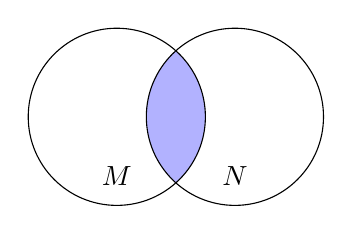
\begin{tikzpicture}[scale=.75]
                \begin{scope}
                \clip (-1,0) circle (1.5cm);
                \fill[blue!30!white] (1,0) circle (1.5cm);
                \end{scope}
                \draw (-1,0) circle (1.5cm) (-1,-1) node {$M$} (1,0) circle (1.5cm) (1,-1) node {$N$};
            \end{tikzpicture}
            \caption{Schnitt $M\cap N$}
        \end{minipage}
        \quad
        \begin{minipage}{.48\textwidth}
            \centering
            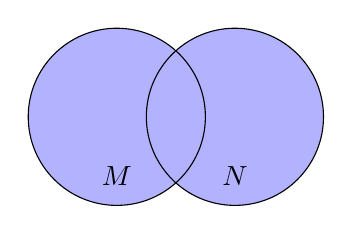
\begin{tikzpicture}[scale=.75]
                \filldraw[fill=blue!30!white, draw=black] (-1,0) circle (1.5cm) (-1,-1) node {$M$} (1,0) circle (1.5cm) (1,-1) node {$N$};
            \end{tikzpicture}
            \caption{Vereinigung $M\cup N$}
        \end{minipage}
        \quad\\[1em]
        \begin{minipage}{.48\textwidth}
            \centering
            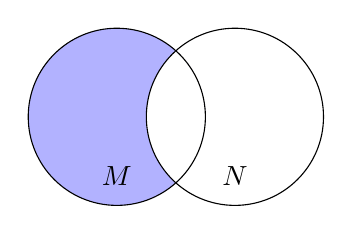
\begin{tikzpicture}[scale=.75]
                \fill[blue!30!white] (-1,0) circle (1.5cm);
                \begin{scope}
                \clip (-1,0) circle (1.5cm);
                \fill[white] (1,0) circle (1.5cm);
                \end{scope}
                \draw (-1,0) circle (1.5cm) (-1,-1) node {$M$} (1,0) circle (1.5cm) (1,-1) node {$N$};
            \end{tikzpicture}
            \caption{Differenz $M\setminus N$}
        \end{minipage}
        \quad
        \begin{minipage}{.48\textwidth}
            \centering
            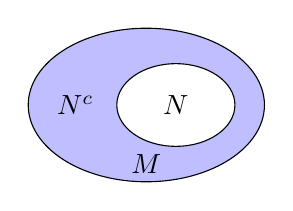
\begin{tikzpicture}[scale=.75]
                \filldraw[fill=blue!25!white, draw=black] (0,0) ellipse (2cm and 1.3cm);
                \filldraw[fill=white!25!white, draw=black] (.5,0) ellipse (1cm and .7cm);
                \path (-1.2,0) node {$N^c$} (0,-1) node {$M$} (.5,0) node {$N$};
            \end{tikzpicture}
            \caption{Komplement von $N$ in $M$}
        \end{minipage}
    \end{figure}
\end{de}


\begin{bsp} \quad
    \begin{enumerate}
        \item Seien $ M = \{1, 2, 4\}$ und $N = \{1, 4, 7\}$. Dann gilt: 
	\begin{align*}
            M \cap N &= \{1, 4\} & M \cup N &= \{1, 2, 4, 7\} & M \setminus N &= \{2\}
	\end{align*}
        \item Für eine natürliche Zahl $n\in \N$ bezeichne
            \[ n\Z := \{ m\in \Z \mid \exists k\in \Z:\ m=kn \} \]
        die Menge aller ganzzahligen Vielfachen von $n$, d.h. aller ganzen Zahlen, die durch $n$ teilbar sind. Dann wurde in \cref{bsp:hinruck} bewiesen, dass
            \[ 2\Z \cap 3\Z = 6\Z \]
        Allgemein gilt für natürliche Zahlen $n,m\in \N$, dass $n\Z\cap m\Z = \kgV(n,m)\Z$, wobei „$\kgV(n,m)$“ das kleinste gemeinsame Vielfache von $n$ und $m$ bezeichnet.
    \end{enumerate}
\end{bsp}


\begin{de}[Mengenfamilie] \index{Mengenfamilie}
    Eine \textbf{Mengenfamilie} (oder auch: \emph{Familie von Mengen}) ist eine Familie, deren Einträge allesamt Mengen sind.
\end{de}


\begin{bsp}
    Beispielsweise ist $(\{1,\dots , n\})_{n\in \N}$ eine Familie von Teilmengen von $\N$, deren Einträge genau die „Anfangsabschnitte“ von $\N$ sind.
\end{bsp}


\begin{de}[Schnitte und Vereinigungen beliebig vieler Mengen] \label{def:mehrfachcapcup}
    Sei $(M_i)_{i\in I}$ eine Familie von Mengen. Es heißen
    \begin{align*}
        \bigcap_{i\in I} M_i &:= \{x \mid \forall i\in I:\ x\in M_i\} & \bigcup_{i\in I}M_i &:= \{x \mid \exists i\in I:\ x\in M_i\}
    \end{align*}
    der \textbf{Durchschnitt} und die \textbf{Vereinigung} der $M_i$'s.
    
    Ist $M$ eine Menge, deren Elemente ebenfalls allesamt Mengen sind, so heißen
    \begin{align*}
        \bigcap M & := \{ x \mid \forall m\in M:\ x\in m \} & \bigcup M & := \{x\mid \exists m\in M:\ x\in m \}
    \end{align*}
    der \emph{Durchschnitt} und die \emph{Vereinigung} von $M$.
\end{de}


\begin{nota} \label{alternativmehrfachcapcup}
    Ist die Indexmenge von der Form $I=\{1,2,\dots,n\}$ für eine natürliche Zahl $n\in \N$, so schreibt man alternativ:
    \begin{align*}
        M_1\cap M_2\cap\ldots\cap M_n & := \bigcap_{i=1}^n M_i := \bigcap_{i\in \{1,\dots , n\}} M_i\\
        M_1\cup M_2\cup\ldots\cup M_n & := \bigcup_{i=1}^n M_i := \bigcup_{i\in \{1,\dots , n\}} M_i
    \end{align*}
\end{nota}


\begin{bsp}
    Sei $H$ die Menge aller Lustigen Taschenbücher und für $h\in H$ sei $L_h$ die Menge aller Menschen, die das Comicbuch $h$ gelesen haben. Dann ist $\bigcap_{h\in H} L_h$ die Menge aller Leute, die \emph{jedes} LTB gelesen haben. Dagegen ist $\bigcup_{h\in H} L_h$ die Menge aller Leute, die mindestens einmal ein LTB gelesen haben.
\end{bsp}


\begin{bem}[Mengen-Operatoren vs. Aussagen-Operatoren]
    Die Operationen $\cap$ und $\cup$ sind in gewisser Weise mengentheoretische „Realisierungen“ der aussagenlogischen Junktoren $\land$ und $\lor$. Deshalb sehen sich auch die Zeichen so ähnlich. Trotzdem solltest du $\cap$ und $\cup$ sorgfältig von $\land$ und $\lor$ unterscheiden: Der Ausdruck „$M\cap N$“ ergibt nur Sinn, wenn $M$ und $N$ Mengen sind; der Ausdruck „$A\wedge B$“ dagegen nur, wenn $A$ und $B$ Aussagen sind. Für zwei Mengen $M,N$ ist „$M\land N$“ kein sinnbehafteter Ausdruck!
    \[\begin{tabular}{c|c|c|c|c|c}
        Mengenoperation & $M\cap N$ & $M\cup N$ & $N^c$ & $\bigcap_{i\in I} M_i$ & $\bigcup_{i\in I} M_i$ \\ \midrule
        Logikoperation & $A\land B$ & $A \lor B$ & $\neg B$ & $\forall x: E(x)$ & $\exists x: E(x)$
    \end{tabular}\]
\end{bem}


\subsection*{Produkt}


\begin{de}[Produkte von Mengen] \index{Produkt von Mengen} \index{Kartesisches Produkt}
    Sei $(M_i)_{i\in I}$ eine Familie von Mengen. Die Menge
        \[ \prod_{i\in I} M_i := \{ (a_i)_{i\in I} \mid \forall i\in I:\ a_i\in M_i \} \]
    aller durch $I$ indizierten Familien, an deren $i$-ter Stelle jeweils ein Element aus $M_i$ steht, heißt das \textbf{(kartesische) Produkt} der $M_i$'s.

    Ist die Indexmenge von der Gestalt $I=\{1,\dots , n\}$ für eine natürliche Zahl $n$, so schreibt man auch
        \[ M_1\times\ldots\times M_n := \prod_{i=1}^n M_i := \prod_{i\in \{1,\dots , n\}} M_i   \]
    Per Definition ist
        \[ M_1\times\ldots\times M_n = \{ (x_1,\dots , x_n) \mid x_1\in M_1,\ \ldots,\ x_n\in M_n \} \]
    d.h. bei $M_1\times\ldots\times M_n$ handelt sich um die Menge aller $n$-Tupel, deren $i$-ter Eintrag ($i\in \{1,\dots , n\}$) jeweils ein Element von $M_i$ ist.
    Insbesondere ist für zwei Mengen $M$ und $N$
    \begin{align*}
        M \times N & = \left\{ (x,y) \mid x\in M\ \text{und}\ y\in N \right\}  && (\text{lies: „$M$ kreuz $N$“})
    \end{align*}
    die Menge aller geordneten Paare, deren erster Eintrag aus $M$ und deren zweiter Eintrag aus $N$ stammen. Man spricht vom \emph{(kartesischen) Produkt} von $M$ und $N$.
\end{de}


\begin{bsp} \quad
    \begin{enumerate}
        \item Es ist
            \[ \{2,3,4\}\times \{ \clubsuit,\heartsuit\} = \{ (2,\clubsuit), (3,\clubsuit), (4,\clubsuit), (2,\heartsuit), (3,\heartsuit), (4,\heartsuit) \}\]
        \item Es ist $\R\times \R=\R^2$ und die Elemente von $\R\times \R$ können als Koordinaten von Punkten in der Ebene interpretiert werden. Die Idee, Punkte mithilfe von Koordinatensystemen und geometrische Figuren als Lösungsmengen von Gleichungen zu beschreiben, wird traditionell Descartes\footnote{\href{https://de.wikipedia.org/wiki/Rene_Descartes}{René Descartes (1596-1650)}} (latinisiert: Cartesius) zugeschrieben. Daher spricht man auch vom \emph{kartesischen} Produkt.
    \end{enumerate}
\end{bsp}


\begin{bsp}[* Matrizen und arrays] \label{bsp:matrizen} \index{Matrix} \quad
    \begin{enumerate}
        \item Seien $m,n\in \N$ und $M=\{1,\dots , m\}$, $N=\{1,\dots,n\}$. Dann ist
            \[ M\times N = \{ (i,j) \in \N\times \N \mid 1\le i\le m \ \text{und}\ 1\le j \le n \} \]
        die Menge aller Paare natürlicher Zahlen, deren erster Eintrag zwischen $1$ und $m$ und deren zweiter Eintrag zwischen $1$ und $n$ liegt.

        Familien mit Indexmenge $M\times N$ werden auch \textbf{($m\times n$)-Matrizen} genannt. Die Einträge einer Matrix werden in einem zweidimensionales Schema (in „Matrixgestalt“) aufgelistet, wobei der erste Index die Zeile und der zweite Index die Spalte markiert:
        \begin{align*}
            \begin{pmatrix}
                a_{11} & \cdots & a_{1n} \\
                \vdots && \vdots \\
                a_{m1} & \cdots & a_{mn}
            \end{pmatrix}
        \end{align*}
        Ist $M$ irgendeine Menge, so wird mit
        \begin{align*}
            M^{m\times n} := M^{\{1,\dots , m\}\times \{1,\dots , n\}}
        \end{align*}
        die Menge aller $(m\times n)$-Matrizen mit Einträgen aus $M$ notiert. Beispielsweise ist $\R^{m\times n}$ die Menge aller $(m\times n)$-Matrizen, deren Einträge reelle Zahlen sind. Solche Matrizen sind ein zentrales Studienobjekt der Linearen Algebra.
        \item Seien $n\in \N$, $m_1,\dots , m_n\in \N$ und $M_i:=\{1,\dots , m_i\}$ für $i\in \{1,\dots , n\}$. Eine Familie mit Indexmenge $M_1\times\ldots\times M_n$ kannst du dir als „$n$-dimensionale Matrix“ vorstellen. In der Informatik werden solche Objekte „$n$-dimensionale arrays“ genannt. In der Physik und der multilinearen Algebra werden sie zur Koordinatendarstellung sogenannter „Tensoren“ verwendet.
    \end{enumerate}
\end{bsp}


\begin{bem}[Potenz als Produkt mit sich selbst]
    Seien $I,M$ zwei Mengen und $(M)_{i\in I}$ die „konstante Familie“, die an jedem Eintrag die Menge $M$ stehen hat. Dann ist $\prod_{i\in I} M$ schlicht die Menge $M^I$ aus \cref{def:mengenpotenz}. Ebenso gilt für jede natürliche Zahl $n$:
        \[ M^n = \underbrace{M\times\ldots\times M}_{\text{$n$-mal}} \]
    sodass beispielsweise $\R\times \R\times \R= \R^3$.

    Also ist $M^I$ eine Art „$I$-faches Produkt von $M$ mit sich selbst“, genauso wie für zwei natürliche Zahlen $m,n\in \N$ die Potenz
        \[ m^n := \underbrace{m\cdot\ldots\cdot m}_{\text{$n$-mal}}\]
    das $n$-fache Produkt von $m$ mit sich selbst ist. Aus diesem Grund wird $M^I$ die „$I$-te Potenz von $M$“ genannt.
\end{bem}


\begin{vorschau}[* Auswahlaxiom] \label{auswahlaxiom} \index{Auswahlaxiom} \index{intangible}
    Sind $M,N$ zwei nichtleere Mengen, etwa mit Elementen $x\in M$ und $y\in N$, so ist auch das kartesische Produkt $M\times N$ nichtleer, weil $(x,y)\in M\times N$. Ist dagegen $(M_i)_{i\in I}$ eine Familie unendlich vieler nichtleerer Mengen, so ist es, sofern keine weiteren Informationen über die Mengen $M_i$ bekannt sind, unmöglich, zu zeigen, dass auch das Produkt $\prod_{i\in I} M_i$ nichtleer ist.

    Sei zum Beispiel $I:= \calP(\R)\setminus \{\emptyset\}$ die Menge aller nichtleeren Teilmengen von $\R$. Du kannst ja mal versuchen, ein konkretes Element von $\prod_{M\in I} M$ hinzuschreiben, was darauf hinausläuft, irgendwie aus jeder nichtleeren Teilmenge von $\R$ ein Element „auszuwählen“.

    Einige (nichtkonstruktive) Sätze der modernen Mathematik sind nun allerdings darauf angewiesen, dass Produkte beliebig vieler nichtleerer Mengen stets nichtleer sind. Daher bildet genau diese Aussage ein eigenes Axiom, das sogenannte \href{https://en.wikipedia.org/wiki/Axiom_of_choice}{Auswahlaxiom}.

    Es lässt sich zeigen, dass es selbst mit Auswahlaxiom unmöglich ist, ein konkretes Element des Produkts $\prod_{M\in \calP(\R)\setminus \{\emptyset\}} M$ hinzuschreiben. Daher handelt es sich um ein \emph{nichtkonstruktives} Axiom: es behauptet die Existenz eines Elements, ohne eine Anleitung für dessen Konstruktion an die Hand zu geben.\footnote{In der sogenannten „konstruktiven Mathematik“ (vgl. \cref{nichtkonstruktiv}) wird das Auswahlaxiom daher nicht akzeptiert. Im mathematischen Mainstream, dem auch die Vorlesungen folgen, wird es dagegen bedenkenlos eingesetzt.} Mathematische Objekte, deren Existenz zwar abstrakt bewiesen werden kann, die sich aber nicht konkret beschreiben oder konstruieren lassen, werden im Englischen auch ``intangibles'' genannt. Beispielsweise handelt es sich bei den Elementen von $\prod_{M\in \calP(\R)\setminus \{\emptyset\}} M$ um intangibles.
\end{vorschau}





\subsection*{* Disjunkte Vereinigung}


\begin{de}[Disjunktheit] \label{def:disjunkt} \index{disjunkte Mengen}
    Zwei Mengen $M,N$ heißen \textbf{disjunkt}, wenn sie keine gemeinsamen Elemente haben, also wenn $M\cap N=\emptyset$.

    Eine Familie von Mengen $(M_i)_{i\in I}$ heißt \textbf{paarweise disjunkt}, wenn je zwei der $M_i$'s disjunkt sind, d.h. wenn gilt:
    \begin{align*}
        M_i\cap M_j \neq  \emptyset \quad& \to\quad i=j &&\text{für alle $i,j\in I$}
    \end{align*}
    Sind $M,N$ zwei disjunkte Mengen, so wird deren Vereinigung auch eine \textbf{disjunkte Vereinigung} genannt und mit
    \begin{align*}
        M\ \dot\cup\ N & := M\cup N && (\text{sofern $M,N$ disjunkt sind})
    \end{align*}
    notiert. Beachte, dass „$\dot\cup$“, anders als es der Vergleich mit \cref{entwederoder} vielleicht nahelegt, keine neue Mengenoperation darstellt, sondern schlicht die Vereinigung aus \cref{def:capcup} gemeint ist. Der Punkt dient lediglich als Mitteilung darüber, dass die beiden Mengen, von deren Vereinigung die Rede ist, disjunkt sind.

    Ebenso wird die Vereinigung einer Familie $(M_i)_{i\in I}$ paarweiser disjunkter Mengen deren \emph{disjunkte Vereinigung} genannt. Man schreibt:
    \begin{align*}
        \dot{\bigcup_{i\in I}}\ M_i & := \bigcup_{i\in I} M_i && (\text{sofern die $M_i$'s paarweise disjunkt sind})
    \end{align*}
\end{de}


\begin{bsp} \label{bsp:disjunkt} \quad
    \begin{enumerate}
        \item Die Mengen $\{\text{Spieler der TSG Hoffenheim}\}$ und $\{\text{Spieler des FSV Mainz 05}\}$ sind disjunkt, weil kein Spieler zugleich bei beiden Vereinen verpflichtet ist.
        \item Die Mengen $\{\text{Informatikstudenten}\}$ und $\{\text{Mathestudenten}\}$ sind nicht disjunkt, weil manche Leute auch beide Fächer zugleich studieren.
        \item Es ist
        \begin{align*}
        \{1,2,3,4,5\} & = \{1,3,4\}\ \dot\cup\ \{2,5\} \\
        \Z & = \{n\in \Z\mid n\ge 0\} \ \dot\cup\ \{n\in \Z\mid n<0\}
        \end{align*}
    \end{enumerate}
\end{bsp}


\begin{bem}
    Die Vereinigung einer paarweise disjunkten Mengenfamilie kannst du dir als eine Art „Addition“ vorstellen. Beispielsweise lässt sich zeigen: sind $n,m\in \N$ und $M$ eine Menge mit $m$-vielen Elementen, $N$ eine zu $M$ disjunkte Menge mit $n$-vielen Mengen, so enthält die disjunkte Vereinigung $M\ \dot\cup\ N$ genau $(m+n)$-viele Elemente.

    Für nicht-disjunkte Vereinigungen gilt das aber nicht. Beispielsweise ist
        \[\{1,3,4\} \cup \{2,3\}= \{1,2,3,4\} \]
    d.h. die Vereinigung einer 2-elementigen Menge mit einer dreielementigen Menge enthält nur vier Elemente.

    Aber auch nicht-disjunkte Mengen können aufeinander „addiert“ werden mithilfe des folgenden Tricks: Ist $(M_i)_{i\in I}$ eine beliebige (nicht notwendig paarweise disjunkte) Mengenfamilie, so sind die Mengen
    \begin{align*}
        \{i\}\times M_i &= \{(i,x) \mid x\in M_i\} && i\in I
    \end{align*}
    paarweise disjunkt. Die Elemente von $\{i\}\times M_i$ kannst du dir vorstellen als die gleichen Elemente wie von $M_i$, nun aber mit einem „Marker“ versehen, der ihre Zugehörigkeit zu $M_i$ kennzeichnet und sie von den Elementen von $\{j\}\times M_j$ für $j\in I\setminus \{i\}$ unterscheidet. Durch den Übergang von $M_i$ zu den $\{i\}\times M_i$ wurden die $M_i$'s „künstlich disjunkt gemacht”. 
\end{bem}


\begin{de}[Disjunkte Vereinigung] \label{def:disjunktcup} \index{Disjunkte Vereinigung}
    Sei $(M_i)_{i\in I}$ eine Familie von Mengen. Die Menge
        \[ \bigsqcup_{i\in I} M_i := \bigcup_{i\in I} (\{i\}\times M_i) = \{(i,x) \mid i\in I,\ x\in M_i \}\]
    heißt die (äußere) \textbf{disjunkte Vereinigung} der $M_i$'s.
    
    Ist die Indexmenge $I$ von der Gestalt $I=\{1,\dots , n\}$ für eine natürliche Zahl $n\in \N$, so schreibt man auch
        \[ M_1\sqcup\ldots\sqcup M_n := \bigsqcup_{i=1}^n M_i := \bigsqcup_{i\in \{1,\dots , n\}} M_i \]
    Insbesondere ist für zwei Mengen $M$ und $N$:
        \[ M\sqcup N = \{ (i,x)\mid i=1\ \text{und}\ x\in M\quad\text{oder}\quad i=2\ \text{und}\ x\in N\} \]
    Man spricht von der \emph{disjunkten Vereinigung von $M$ und $N$}.
\end{de}


\begin{bsp}
    Es ist
        \[\N \sqcup\N=\{(1,1),(1,2),(1,3),(1,4)\dots,(2,1),(2,2),(2,3),(2,4)\dots\} \]
    d.h. die Menge $\N\sqcup \N$ besteht aus zwei „Kopien“ von $\N$. Für jede natürliche Zahl $n$ enthält sie jeweils zwei „Klone“ von $n$, realisiert als $(1,n)$ und $(2,n)$.
    \begin{figure}[ht]
    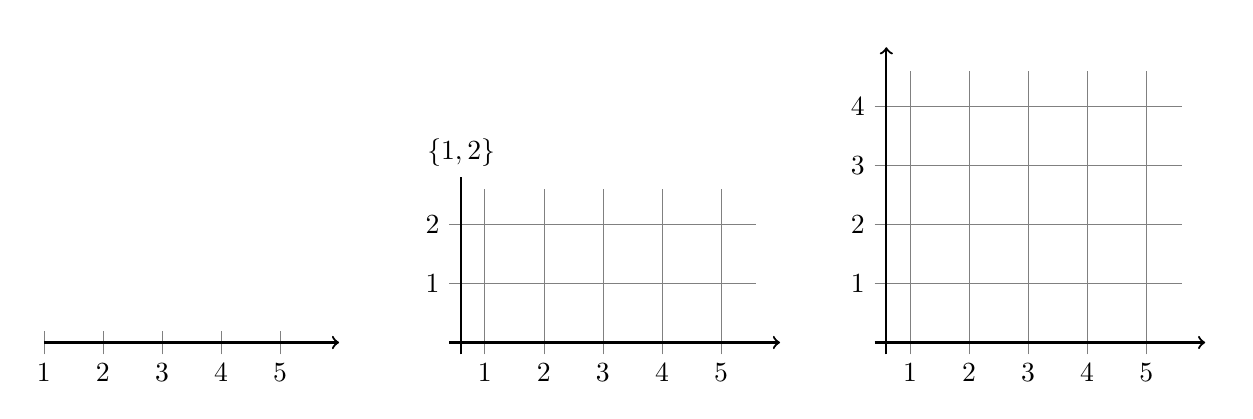
\begin{tikzpicture}
        \begin{scope}[xshift=-5cm,scale=1.5]
            \draw[step=.5cm,style=help lines] (-1,-.1) grid (1.3,.1);
            \draw[->,thick] (-1,0) -- (1.5,0) node[right] {$\N$};
            \foreach \x in {1,2,3,4,5}
            \draw[xshift=.5*\x cm] (-1.5,-.1) node[below] {\x};
        \end{scope}
        \begin{scope}[scale=1.5, xshift= 0.4cm]
            \draw[style=help lines,step=.5 cm] (-1.3,-.1) grid (1.3,1.3);
            \begin{scope}
                \draw[->, thick] (-1.3,0) -- (1.5,0) node[right] {$\N$};
                \draw[thick] (-1.2,-.1) -- (-1.2,1.4) node[above] {$\{1,2\}$} coordinate(y axis);
                \foreach \x in {1,2,3,4,5}
                \draw[xshift=.5*\x cm] (-1.5,-.1) node[below] {\x};
                \foreach \y in {1,2}
                \draw[yshift=.5*\y cm] (-1.3,0) node[left] {\y};
            \end{scope}
        \end{scope}
        \begin{scope}[scale=1.5,xshift=4cm]
            \draw[style=help lines,step=.5 cm] (-1.3,-.1) grid (1.3,2.3);
            \begin{scope}
                \draw[->, thick] (-1.3,0) -- (1.5,0) node[right] {$\N$};
                \draw[->, thick] (-1.2,-.1) -- (-1.2,2.5) node[above] {$\N$} coordinate(y axis);
                \foreach \x in {1,2,3,4,5}
                \draw[xshift=.5*\x cm] (-1.5,-.1) node[below] {\x};
                \foreach \y in {1,2,3,4}
                \draw[yshift=.5*\y cm] (-1.3,0) node[left] {\y};
            \end{scope}
        \end{scope}
    \end{tikzpicture}
    \centering \caption{Vergleich von $\N\cup\N\ (=\N)$, $\N\sqcup\N$ und $\N\times\N$.}
\end{figure}
\end{bsp}
    
    
\begin{bem}[Produkt als Summe mit sich selbst]
    Seien $I,M$ zwei Mengen und $(M)_{i\in I}$ die „konstante Familie“, die an jedem Eintrag die Menge $M$ stehen hat. Dann ist $\bigsqcup_{i\in I} M_i$ genau das kartesische Produkt $I\times M$. Ebenso gilt für jede natürliche Zahl $n$:
        \[ \{1,\dots , n\} \times M = \underbrace{M\sqcup\ldots\sqcup M}_{\text{$n$-mal}} \]
    Also ist $I\times M$ die „$I$-fache Summe von $M$ mit sich selbst“, genauso wie für zwei natürliche Zahlen $m,n\in \N$ das Produkt
        \[ n\cdot m := \underbrace{m +\ldots + m}_{\text{$n$-mal}}\]
    die $n$-fache Summe von $m$ mit sich selbst ist.
\end{bem}


\begin{vorschau}
    Der Ausdruck „disjunkte Vereinigung“ ist nun mit mehreren Bedeutungen „überladen“.
    \begin{enumerate}[(1)]
        \item Zum einen bezeichnet er die disjunkte Vereinigung aus \cref{def:disjunktcup}, also die Konstruktion, mit der Mengen zuerst „künstlich disjunkt“ gemacht und daraufhin „addiert“ werden. Wir haben dafür folgende Notation verwendet:
            \[ M\sqcup N \qquad\text{bzw.}\qquad \bigsqcup_{i\in I} M_i \]
        \item Zum anderen bezeichnet er schlicht die gewöhnliche Vereinigung einer Familie paarweiser disjunkter Mengen, siehe \cref{def:disjunkt}, was wir durch
            \[ M\ \dot\cup\ N \qquad\text{bzw.}\qquad   \dot{\bigcup_{i\in I}}\ M_i \]
        notiert haben.
    \end{enumerate}
    Hinzu kommt, dass in der Literatur beide Notationen durcheinander verwendet werden, d.h. sowohl die Objekte (1) als auch die Objekte (2) werden mal mit „$\dot\cup$“, mal mit „$\sqcup$“ bezeichnet
    
    Tatsächlich ist es in den meisten Fällen auch gar nicht wichtig, wie genau die disjunkte Vereinigung „$M \sqcup N$“ definiert ist, d.h. wie ganau man die Mengen $M,N$ künstlich disjunkt gemacht hat. Die disjunkte Vereinigung bezieht ihre Signifikanz vor allem aus der kategorientheoretischen Eigenschaft, ein sogenanntes \emph{Koprodukt} zu sein. In dieser Hinsicht ist sie ein genaues Gegenstück zum kartesischen Produkt. Mehr darüber wirst du in Vorlesungen und Büchern über Kategorientheorie lernen.
\end{vorschau}





\clearpage
\section{Aufgabenvorschläge}


\begin{aufg}[Kennenlernen]
    Es sei $T$ die Menge aller Leute, die sich gerade in diesem Tutorium befinden.
    Welche der folgenden Mengen sind Teilmengen voneinander? Welche Mengen sind sogar gleich?
    \begin{align*}
        S&:= \{ x\in T \mid x\ \text{ist sportlich} \}  && \emptyset  \\
        N&:=  \{ x\in T \mid x\ \text{geht gern in die Natur} \} && T \\
        W & := \{ x\in T \mid x\ \text{kennt sich auf einem Spezialgebiet richtig gut aus} \} &&  N\setminus S  \\
        M &:= \{ x \in T \mid x\ \text{spielt ein Musikinstrument} \} && W \cup S
    \end{align*}
\end{aufg}


\begin{aufg}[Mengen vs. Familien]
    Es sei $I:=\{1,2,3,4,5\}$ und es sei $a=(a_i)_{i\in I}$ diejenige Familie mit $a_i=i+2$ für jedes $i\in I$. Welche der folgenden Objekte sind einander gleich und welche sind voneinander verschieden?
    \begin{center}
        {\renewcommand{\arraystretch}{1.6}
        \begin{tabular}{ccccccccc}
            $I$ && $(a_i)_{i\in I}$&& $\{a_i\mid i\in I\}$ && $(4,3,5,6,7)$ && $(2,1,3,4,5,5)$ \\
            $a$ && $\{1,2,3,4,5\}$ && $(3,4,5,6,7)$ && $\{4,3,5,6,7\}$ && $\{2,1,3,4,5,5\}$
	\end{tabular}}
    \end{center}
\end{aufg}


\begin{aufg}[Elemente und Teilmengen]
    Beurteilt für jede der folgenden Aussagen, ob sie wahr oder falsch ist:
    \begin{align*}
        \N&  \in \N & \N & \subseteq \N & \N & \in \calP(\N) &  \N & \subseteq \calP(\N) \\
        \N & \in \{ \N\} & \N & \subseteq \{ \N\} & \{ \N\} & \in \{ \N\} & \{\N\} & \subseteq \{ \N\} \\
        \{\N\} & \in \calP(\N) & \{ \N\} & \subseteq \calP(\N) & \calP(\N) & \in \calP(\N) & \calP(\N) & \subseteq \calP(\N) \\
        \emptyset & \in \emptyset & \emptyset &\subseteq \emptyset & \emptyset & \in \calP(\emptyset) & \{\emptyset\} & = \calP(\emptyset)
    \end{align*}
\end{aufg}


\begin{aufg}[Produkte konkret]
    Wir betrachten die Mengen $T := \{ \text{Dr.} \}, A := \{ \text{Herr, Frau} \}$, $V:= \{ \text{Anne, John} \}$ und $N := \{ \text{Hathaway, Sinclair, Wayne} \}$. Listet die Elemente der folgenden Mengen auf:
    \begin{enumerate}
	\item $A \times N$
	\item $A\times T \times V\times N$
	\item $(T \cup V) \times N$
	\item $(T\times N)\cup (V\times N)$
    \end{enumerate}
\end{aufg}


\begin{aufg}[Einige Rechenregeln für $\cap$ und $\cup$] \label{aufg:capcupgesetze}
    Seien $X,Y,Z$ drei beliebige Mengen. Vollzieht die folgenden Gleichungen nach:
    \begin{align*}
        \begin{split}
            (X \cap Y) \cap Z & = X \cap (Y \cap Z) \\
            (X \cup Y) \cup Z & = X \cup (Y \cup Z)
        \end{split}
        && (\text{Assoziativgesetze}) \\[1em]
        \begin{split}
            X \cap (Y \cup Z) & = (X\cap Y) \cup (X\cap Z) \\
            X \cup (Y\cap Z) & = (X\cup Y) \cap (X\cup Z)
        \end{split}
        && ( \text{Distributivgesetze}) 
    \end{align*}
    (Eine lange Liste mit weiteren Rechenregeln für Mengen befindet sich in \cref{formelsammlung}.)
\end{aufg}

